\documentclass[a4paper, 10pt]{article}
\usepackage{amsmath}
\usepackage[a4paper, margin=1.5cm]{geometry}
\usepackage{graphicx}
\begin{document}


+ El mensaje se codifica en la amplitud A(t). $$ A(t) = A_c m(t) \quad\quad \phi(t)= cte \leftarrow \text{por simplicidad igualamos a 0}$$

\begin{figure}[!h]
    \centering
    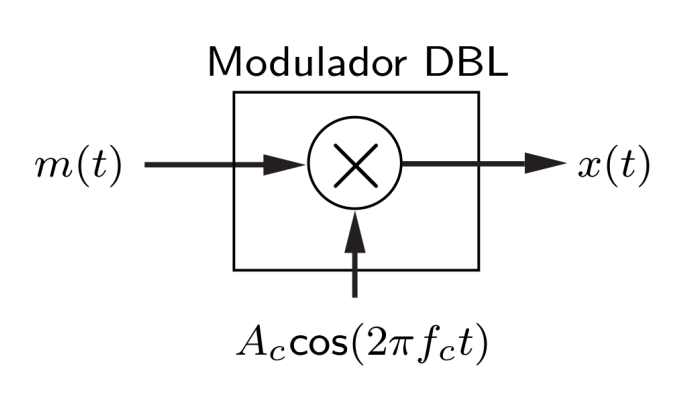
\includegraphics[scale = 0.5]{./modulador.png}
    $$x_{DBL}(t) = Re \{ A_c m(t) e^{j \pi f_ct} \} = A_c m(t) cos(2 \pi f_c t)$$
    $$ x_{DBL}(f) = A_c m(t) * \frac{[\delta(f+f_c) + \delta(f-f_c)]}{2} = \frac{A_c}{2} [m(f+f_c) + m(f-f_c)] $$
\end{figure}

+ Si $m(t)$ es una señal de tipo pasa bajos de ancho de banda $W$, $x_{DBL}(t)$ ocupa el doblde de banda, osea $2W$

+ La portadora no se transmite, se ve en la ausencia de deltas en $f_c$.

+ Para procesos ESA, lo resultados son analogos.

\end{document}
